\subsection{Mendaftarkan Barang untuk Dilelang}
\label{kasus-penggunaan-daftarbarang}
Halaman ini hanya dapat diakses oleh pengguna yang sudah terdaftar dan sudah \textit{login} ke dalam sistem. Halaman ini menampilkan \textit{form} berisi elemen \textit{input} informasi barang, dan pengguna dapat mengisi lalu mengklik tombol tambahkan barang, dan untuk kasus normal dan alternatif dapat dilihat pada Tabel \ref{uc03.01}.\\
\indent Terdapat logika \textit{view} khusus pada implementasi kasus penggunaan ini, karena adanya kebutuhan untuk \textit{upload multiple images} untuk setiap barang dan adanya penggunaan layanan pihak ketiga (AWS Storage Service) sebagai tempat penyimpanan gambar. Kode-kode sumber terkait dengan implementasi kasus penggunaan Mendaftarkan Barang untuk Dilelang adalah sebagai berikut:
	\begin{enumerate}
		\item Logika \textit{back-end} ditulis menggunakan PHP yang dicantumkan dalam Kode Sumber \ref{cdjq.03-01}; 
		\item Logika \textit{view} ditulis menggunakan jQuery yang dicantumkan dalam Kode Sumber \ref{cdjq.03-01}; dan
		\item Logika \textit{upload}/\textit{storage} data gambar, yang ditulis menggunakan PHP dicantumka pada Kode Sumber \ref{cdaws.03-01}
	\end{enumerate} 

  \begin{figure}[H]
    \centering
    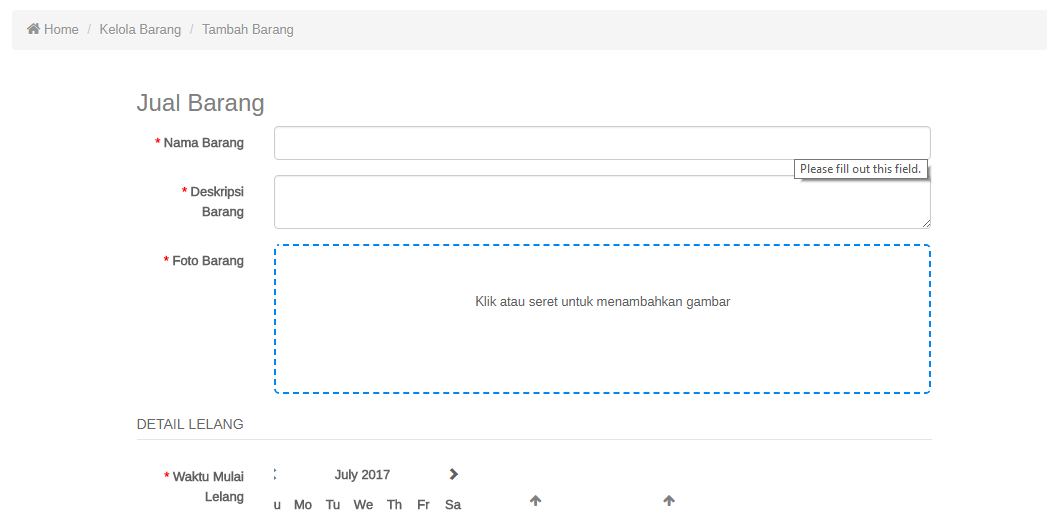
\includegraphics[width=\textwidth]{images/bab4/ui/03-01.png}
    \caption{Halaman Antarmuka Mendaftarkan Barang untuk Dilelang}
    \label{ui.03-01}
  \end{figure}

\newpage
 \begin{lstlisting}[label=cdbe.03-01,style=php,caption=Implementasi \textit{Back-end} Mendaftarkan Barang untuk Dilelang]
/*
    Fungsi create() dipanggil untuk menampilkan halaman tambah barang
    Fungsi store() dipanggil saat form di halaman tambah barang diklik
    File : ItemController
*/
public function create(){
    /*  method : GET */
    return view('pages.'.$this->pageFolder.'.create', $data);
}


/*
    Fungsi store() dipanggil oleh ajax lewat jQuery
    untuk memvalidasi dan insert data ke dalam database
*/
public function store(Request $request)
{
    /*  method : POST */
    $unserialize = $this->unserializeForm($request['data']);
    /*  Validating data */
    $validate = Validator::make($unserialize, $this->itemRep->rules(), $this->itemRep->messages());

    if(false){
        /* Jika gagal, return false dan error message */
        return ['success'=>false, 'msg' => $validate->messages()];
    }
    else{
	    /* Jika sukses, return true 
	    dan id barang yang berhasil diinsert
	       untuk selanjutnya diproses oleh browser
	       untuk upload gambar barang ke URL terpisah.
	     */
	    return ['success' => true, 'id' =>  10];
    }
}
	  
	  
\end{lstlisting}

\begin{lstlisting}[label=cdjq.03-01,style=php,caption=Implementasi \textit{Back-end} Mendaftarkan Barang untuk Dilelang]
/*	Fungsi ini berfungsi untuk \textit{update} gambar barang, diteruskan kepada \textit{script} terpisah 
    Pada file : ImageController
*/
public function uploadItemImage(Request $request){
    //passed here if csrf token is already passed
    $_POST['image'] = $request->file('image');
    $_POST['id_user'] = Auth::user()->id;
    $_POST['ext'] = $request->file('image')->extension();
    require ('/home/img/upload-aws.php');
    return $res;
}
\end{lstlisting}


\begin{lstlisting}[label=cdaws.03-01,style=php,caption=Implementasi \textit{Back-end} \textit{Upload} Gambar Barang]
/*	Fungsi ini berfungsi untuk \textit{upload} gambar lewat script terpisah (untuk alasan integrasi data dengan sistem yang dibuat oleh partner tugas akhir)
*/
require 'vendor/autoload.php';

use Aws\S3\S3Client;

$collection = (new MongoDB\Client("mongodb://127.0.0.1:27017"))->lelangkita->itemimages;
if ($_SERVER['REQUEST_METHOD']=='POST'){
	$image = $_POST['image'];
	$userid = $_POST['id_user'];
	$ext = $_POST['ext'];
	$itemid = $_POST['itemid'];
	$isMainImage = false;
	
	if (isset($_POST['is_main_image']) && !empty($_POST['is_main_image']) && $_POST['is_main_image'] == "true") {
	        $isMainImage = true;
	}
	
	$year = date("Y");
	$month = date("m");
	$date = date("d");
	$unique = uniqid();
	$filename = $userid."_".$unique.".".$ext;
	$path = "img/".$year."/".$month."/".$date."/".$userid;
	$imgpath = $path."/".$filename;

  $decoded_image = base64_decode($image);

  try {
    $s3client = S3Client::factory(array(
      'credentials' => array(
        'key' => 's3\_key\_credentials',
        'secret' => 's3\_secret\_credentials'
      ),
      'profile' => 's3\_profile',
      'region' => 's3\_selected\_server\_regopm'
    ));

    $upload = $s3client->putObject(
      array(
        'Bucket' => 'img-s7.lelangapa.com',
        'Key' => $imgpath,
        'Body'   => $decoded_image,
        'ContentEncoding' => 'base64',
        'ContentType' => 'image/'.$ext,
        'ACL'    => 'public-read'
      )
    );

    $insertToDB = $collection->insertOne([
            'item_id' => $itemid,
            'url' => $imgpath,
                    'is_main_image' => $isMainImage
    ]);

    if ($isMainImage == true) {
	    $indexImageURL = "https://src-api.lelangapa.com/apis/index/submit/image";
	    $headers = array(
	      'Content-Type: application/json'
	    );
	    $post_data = array(
	            "id_item" => $itemid,
	            "main_image_url" => $imgpath
	    );
	    $ch = curl_init();
	    curl_setopt($ch, CURLOPT_URL, $indexImageURL);
	    curl_setopt($ch, CURLOPT_HTTPHEADER, $headers);
	    curl_setopt($ch, CURLOPT_RETURNTRANSFER, 1);
	    curl_setopt($ch, CURLOPT_POST, true);
	    curl_setopt($ch, CURLOPT_POSTFIELDS, json_encode($post_data));
	    curl_setopt($ch, CURLOPT_SSL_VERIFYPEER, FALSE);
	    $indexresult = curl_exec($ch);
	    curl_close($ch);
    }

    if ($upload) {
      $res = array('status' => 'success', 'result' => '1');
                echo "success";
    }
    else {
      $res = array('status' => 'failed', 'result' => '0');
                echo "Failed";
    }
  }
  catch(Exception $e) {
    exit($e->getMessage());
  }
}

\end{lstlisting}